I have tried various methods for estimating the position of the drone system
-- particularly with the goal of determining the velocity of the drone in order to remove the bouncing
that the DecaWave system exhibits.
I initially tested these sensors in isolation to determine which is the most viable,
and therefore where I should most apply my efforts.
It is especially important to note that indoor environments are quite variable,
and not all sensors are applicable to all environments.
In this section I explain the exploratory tests to determine which sensors are viable in V207,
and I discuss the possible factors influencing their behavior.

\subsection{Optical Flow}

The first sensor in the experiments is an ArkFlow optical flow sensor (See Figure~\ref{figure:arkflow_mount}),
which determines x/y-velocity using pixel velocity in a downward-facing camera.
This sensor is used in GPS-denied drone flight to extract velocity information from the
relative movement of the terrain beneath the drone.

\begin{figure}
	\centering
	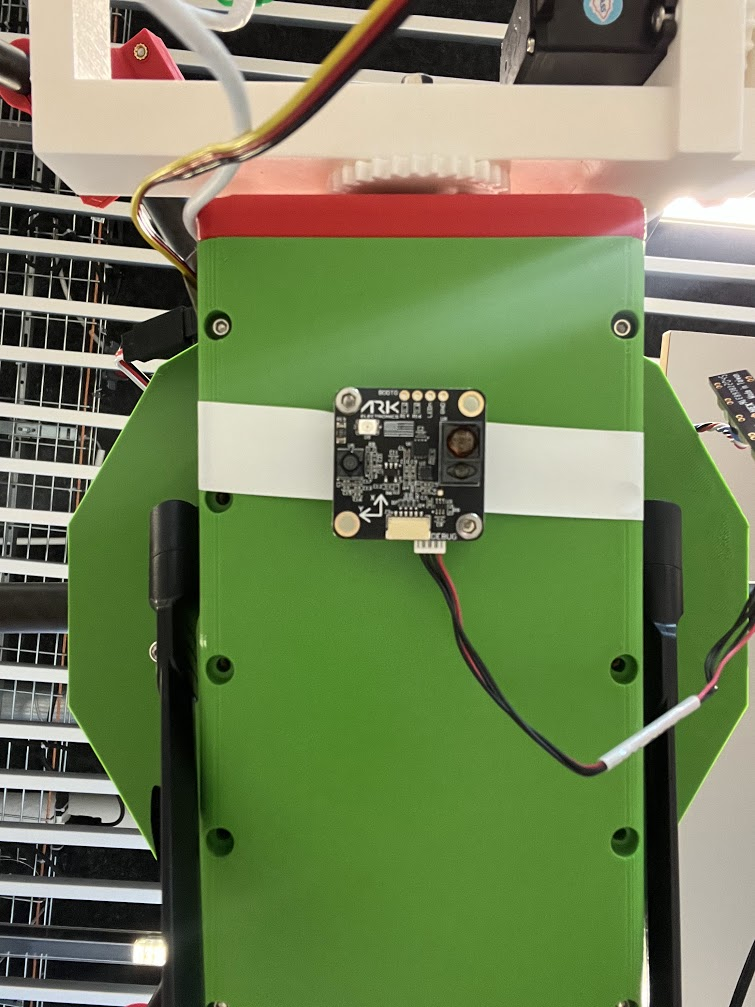
\includegraphics[width=0.5\linewidth]{./images/arkflow_mount}
	\caption{The ArkFlow sensor mounted to the bottom of the drone.}
	\label{figure:arkflow_mount}
\end{figure}

Initial tests show that the sensor is able to perceive motion from a pixel environment
with some variance.
Its raw data is also in some abstract form that must be processed by the flight controller unit (FCU)
before use.
Therefore, the velocity estimate from this sensor came from the FCU directly.
Ultimately, it also has difficulty determining its velocity from the very self-similar floor of V207
(See Figure~\ref{figure:laser}).
Figure~\ref{figure:arkflow_performance_velocity} and~\ref{figure:arkflow_performance_position} show
the noisy velocity and position estimates respectively.
The velocity signal shows a sharp discontinuity in $t\in[65, 74]$,
and a large negative spike at $t=50$,
both of which do not correspond to the reality of the exploratory test.
These are made clearer by the position estimate in Figure~\ref{figure:arkflow_performance_position},
which essentially shows teleportation.
It is possible that this is not only due to the ArkFlow sensor, but also to the FCU's data fusion methods.
However, given time limitations, this method was not explored further.

\begin{figure}
	\centering
	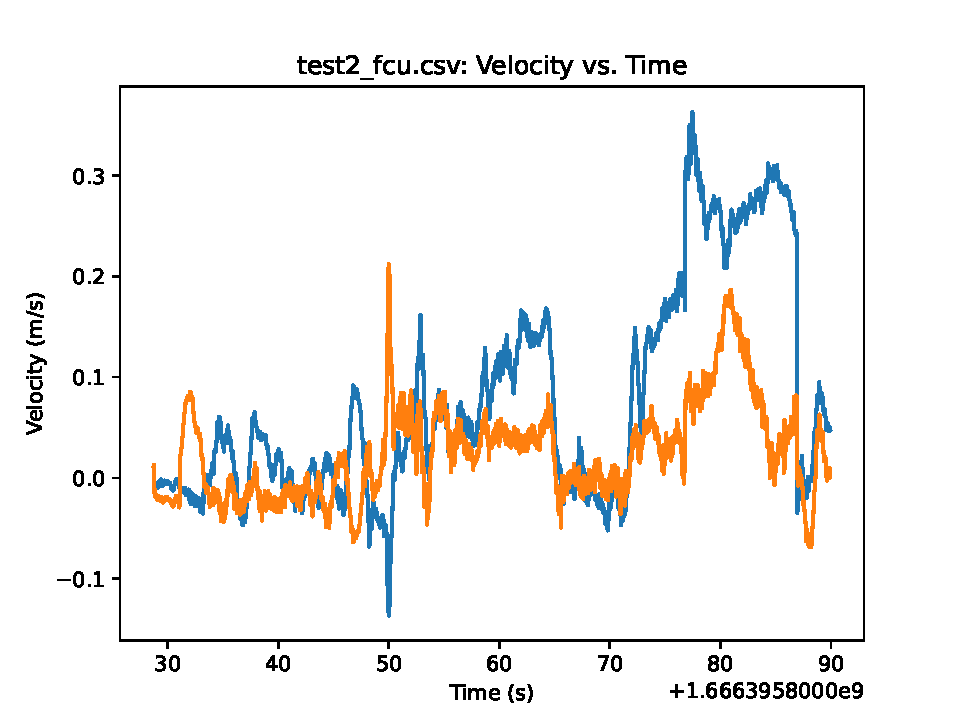
\includegraphics[width=\linewidth]{./images/test2_fcu_velocity}
	\caption{The velocity estimate from the FCU, fusing the ArkFlow data with IMU. Blue and orange correspond to the $x$ and $y$ dimensions respectively.}
	\label{figure:arkflow_performance_velocity}
\end{figure}

\begin{figure}
	\centering
	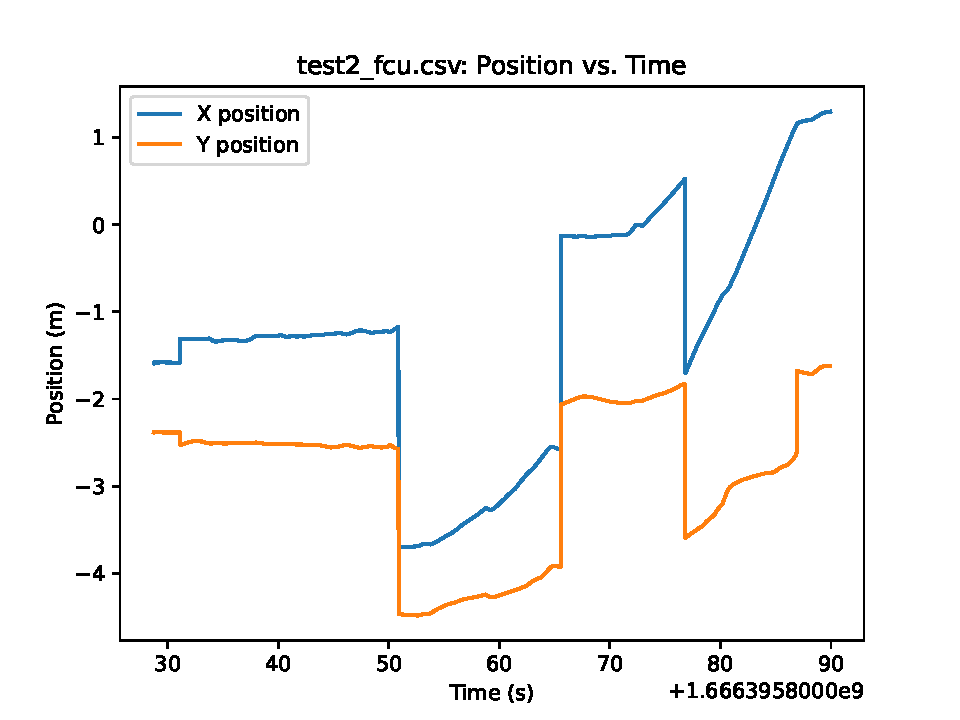
\includegraphics[width=\linewidth]{./images/test2_fcu_position}
	\caption{The position estimate from the FCU, fusing the ArkFlow data with IMU. Blue and orange correspond to the $x$ and $y$ dimensions respectively.}
	\label{figure:arkflow_performance_position}
\end{figure}

\subsection{Depth Flow}

A D455 stereo depth camera provides a relatively clean 3-dimensional view of the scene
in front of the drone.
Let $d_{r,i}$ represent the $i^\mathrm{th}$ \emph{raw} 640x480 depth image
generated from the D455 camera at index $i$.
This is referred to as \emph{raw} because its data is scalar multiples of some \texttt{depth\_scale} $s$
that is included as metadata, according to standard practices in the \texttt{pyrealsense2} library
that connects Python to the sensor itself.
We convert a \emph{raw} depth image $d_{r,i}$ to a depth image $d_i$ simply by multiplying the image
by the depth scale $s$ after converting it to a Numpy array.
So
$$d_i = d_{r,i} \cdot s$$
where $d_i$ is a \emph{depth image},
$d_{r,i}$ is a \emph{raw depth image},
and $s$ is a \emph{depth scale}.

Then, the velocity at index $i$ -- $v_i$ -- is as such:
$$v_i = \dfrac{d_i - d_{i-1}}{\Delta t}$$
where $t=t_i-t_{i-1}$ is the difference in timestamps between $d_i$ and $d_{i-1}$
At this point, the pixel position of the data is no longer important,
so I reshape the 2D array into a 1D array in order to operate on it more easily.

The edges around objects in the depth image are somewhat noisy and discontinuous,
and this can lead to high perceived pixel velocity in the depth dimension.
To remove this particular type of noise, I simply remove all velocity estimates
above a threshold of 1 m/s magnitude, decreasing the size of the velocity array $v_i$.
The whole velocity vector can then be aggregated into a single measurement using a simple arithmetic mean.

To test the overall performance, I recorded the aggregated velocity measurement over time
and plotted it for easy visualization.

For the first test, shown in Figure~\ref{figure:d455_velocity_still},
I simply left the drone still and recorded the velocity over time.
The plot shows relatively little noise -- less than 5 cm/s.
The second test, shown in Figure~\ref{figure:d455_velocity_quick} correctly depicts
discrete time segments of backwards and forwards motion and stillness.
This method of forward/backward velocity estimation appeared promising enough to use in later experiments.

\begin{figure}
	\centering
	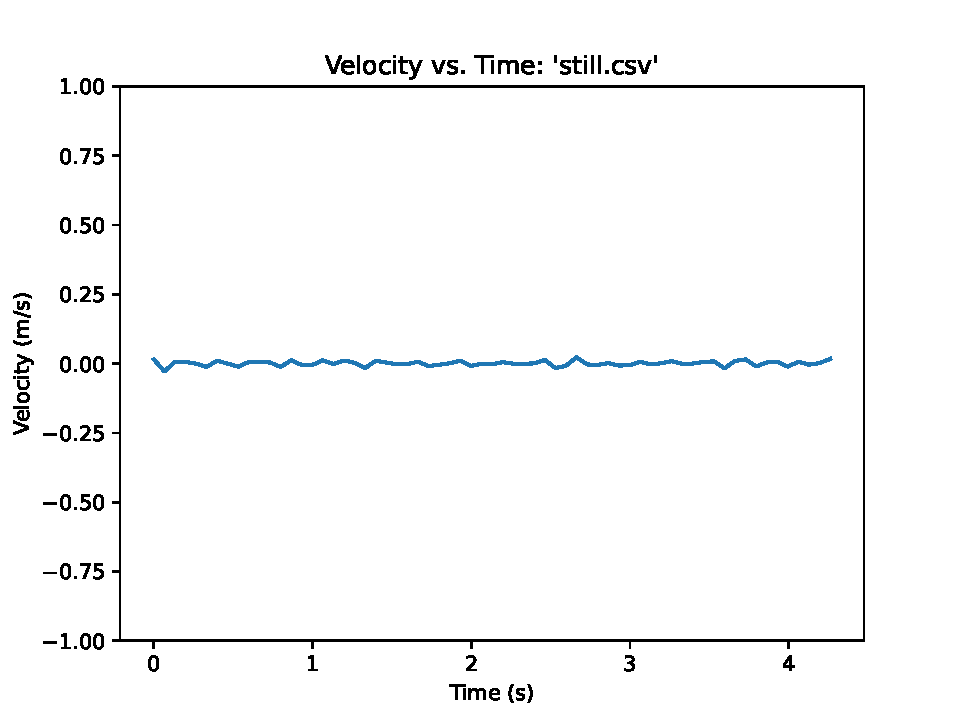
\includegraphics[width=\linewidth]{./images/still.pdf}
	\caption{The perceived velocity while the drone was sitting still.}
	\label{figure:d455_velocity_still}
\end{figure}

\begin{figure}
	\centering
	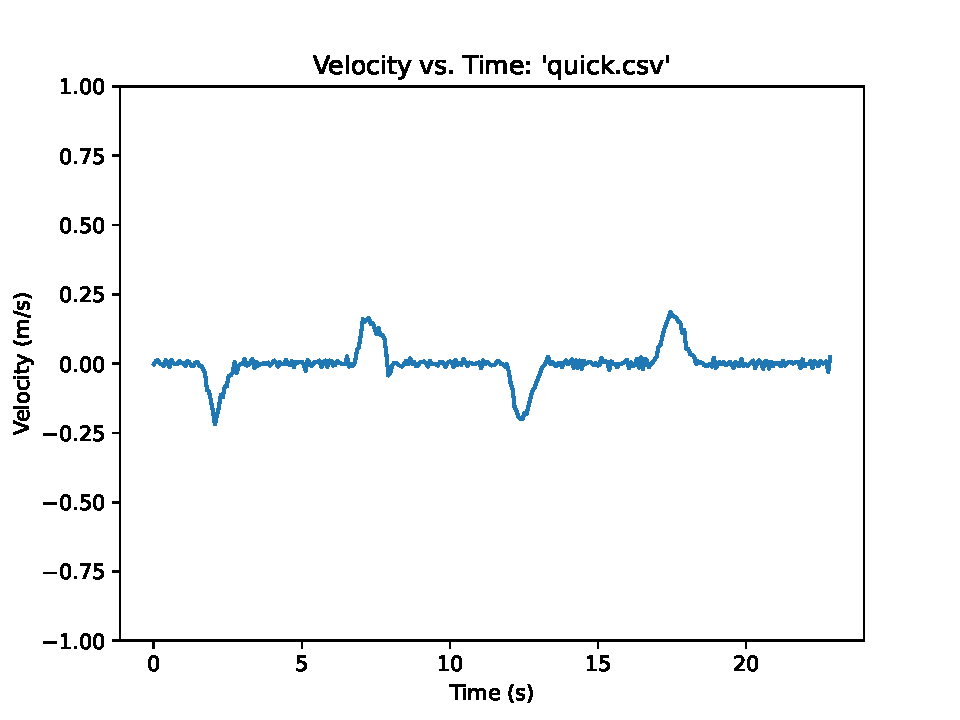
\includegraphics[width=\linewidth]{./images/quick.pdf}
	\caption{The perceived velocity while I moved the drone backwards and forwards quickly twice, leaving it still for a short time between movements.}
	\label{figure:d455_velocity_quick}
\end{figure}

\subsection{Heading Estimation}
\label{section:heading_estimation}

The D455 has an inertial measurement unit with a gyroscope and accelerometer,
for estimation of angular velocity and orientation to the gravity vector.
Given the setup of the testing platform (a pallet jack) one can make the warranted assumption
that the platform must be moving forward/backward or rotating in the yaw dimension only.
Moreover, during testing this is guaranteed by simply constraining the platform to simple movements
that are not antagonistic to the system.
With this assumption, we can use the heading of the drone as a justification to ignore erroneous
motion if it corresponds to the impossible side-to-side motion of the cart.

\begin{figure}
	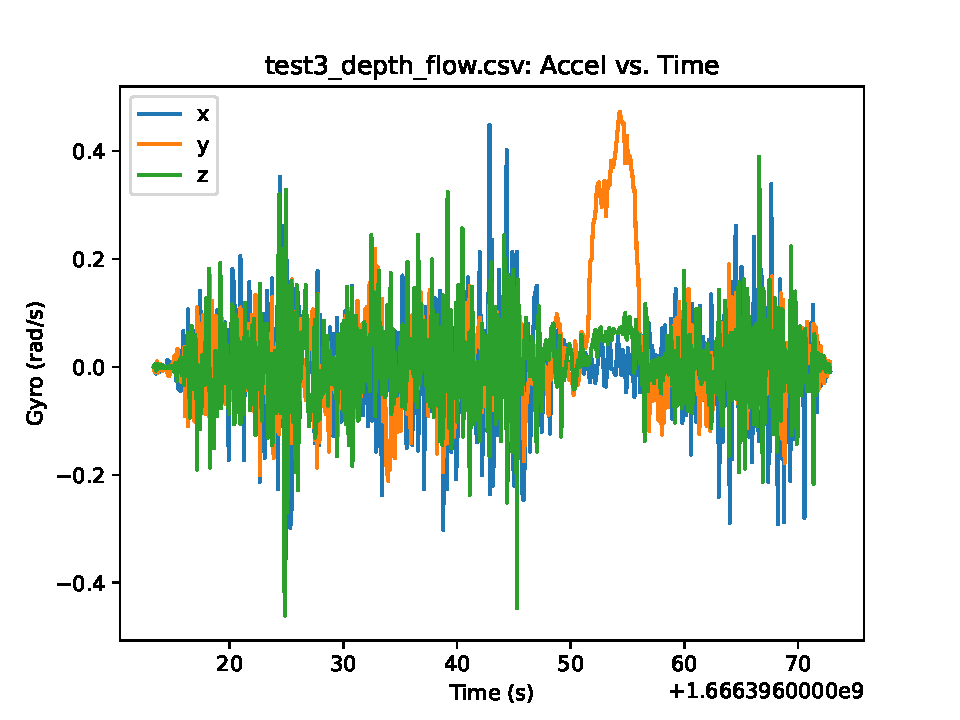
\includegraphics[width=\linewidth]{./images/test3_depth_flow_depth_gyro.pdf}
	\caption{A test of the gyroscope, showing a noise in $x$ and $z$ dimension,
	and a large, correct spike in the $y$ dimension which corresponds to a rotation of the drone
	in the yaw dimension.}
	\label{figure:test3_depth_gyro}
\end{figure}

I have made a Kalman filter to estimate the heading of the drone relative to its starting heading.
Its properties are as below:

Initial state:
$$X_0 =
\left(
\begin{matrix}
	0 & 0
\end{matrix}
\right)
$$

State transition matrix, with a camera framerate of 15 Hz $\rightarrow dt=0.067s$:
$$
F =
\left(
\begin{matrix}
	1 & \frac{1s}{15} \\
	0 & 1
\end{matrix}
\right)
=
\left(
\begin{matrix}
	1 & 0.067 \\
	0 & 1
\end{matrix}
\right)
$$

Measurement model (the gyro measures only speed, and we integrate to get position):
$$H =
\left(
\begin{matrix}
	0 & 1
\end{matrix}
\right)
$$

Covariance matrix:
$$
F =
\left(
\begin{matrix}
	500 & 0\\
	0 & 500
\end{matrix}
\right)
$$

Measurement noise:
$$
R =
\left(
\begin{matrix}
	1000
\end{matrix}
\right)
$$


\subsection{Depth Camera Accelerometer}

Figure~\ref{figure:test2_depth_accel} shows the raw accelerometer data from the D455,
which seems to actually be clean, usable data.
However, all it can really show is that the drone was \emph{relatively} upright for the duration of the tests,
with the Y axis reading roughly $-9.8 \frac{m}{s^2}$, and the X axis hovering around $0 \frac{m}{s^2}$.
The Z axis is slightly negative as a result of the camera (but not the drone) being tilted slightly
downward on its gimbal throughout the tests.

\begin{figure}
	\centering
	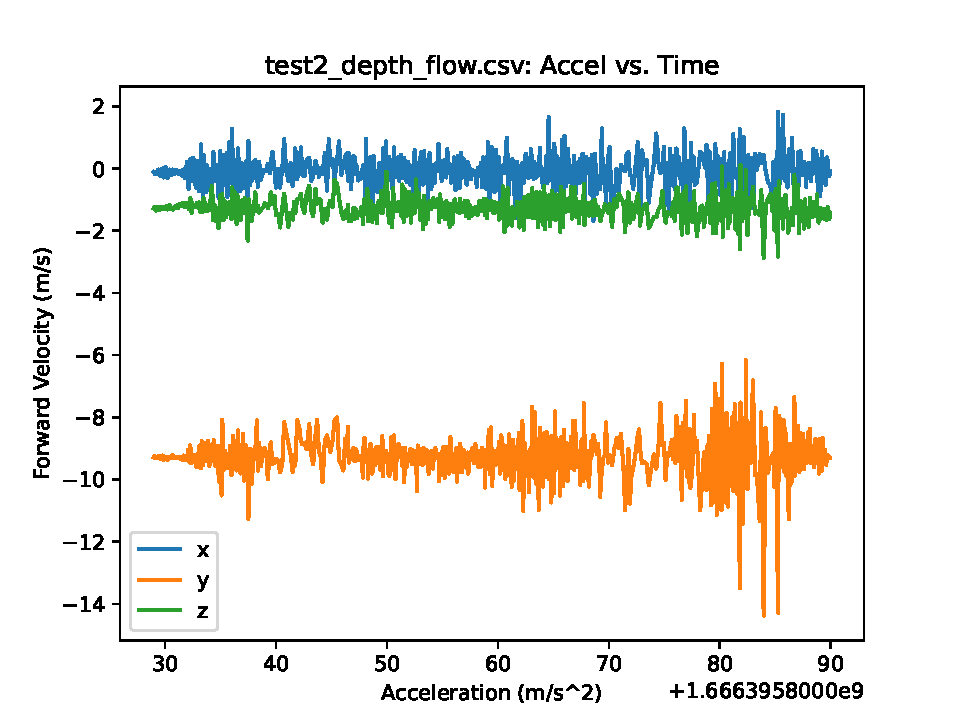
\includegraphics[width=\linewidth]{./images/test2_depth_flow_depth_accel.pdf}
	\caption{Example accelerometer data.}
	\label{figure:test2_depth_accel}
\end{figure}

\subsection{Filtering Methods}

I filter the raw DecaWave data with both a Kalman filter and a sequential importance filter,
to attempt to increase its precision.
Each component of the position $x,y$ uses a single, 1-dimensional filter.
The Kalman filter definition is as below, and differs from the filter in Section~\ref{section:heading_estimation} in that its measurement model specifies that the measurements corresponds to the position,
rather than the velocity, and they are otherwise similar except that one is working in terms of angles
and the other in terms of Cartesian coordinates.

Initial state:
$$X_0 =
\left(
\begin{matrix}
	0 & 0
\end{matrix}
\right)
$$

State transition matrix, with a camera framerate of 15 Hz $\rightarrow dt=0.067s$:
$$
F =
\left(
\begin{matrix}
	1 & d_t \\
	0 & 1
\end{matrix}
\right)
$$

Measurement model (the gyro measures only speed, and we integrate to get position):
$$H =
\left(
\begin{matrix}
	1 & 0
\end{matrix}
\right)
$$

Covariance matrix:
$$
F =
\left(
\begin{matrix}
	5000 & 0 \\
	0 & 5000
\end{matrix}
\right)
$$

Measurement noise:
$$
R =
\left(
\begin{matrix}
	500
\end{matrix}
\right)
$$

The sequential importance filter is implemented exactly as in the file \texttt{sis.py} provided with
the course, but with $n=500$ particles instead of 250.

\subsection{Platform \& Data Collection}

Figure~\ref{figure:testing_platform} shows the data collection platform.
The pallet jack exposes the floor to the optical flow sensor while allowing the drone to 
remain level and unobstructed.

\begin{figure}
	\centering
	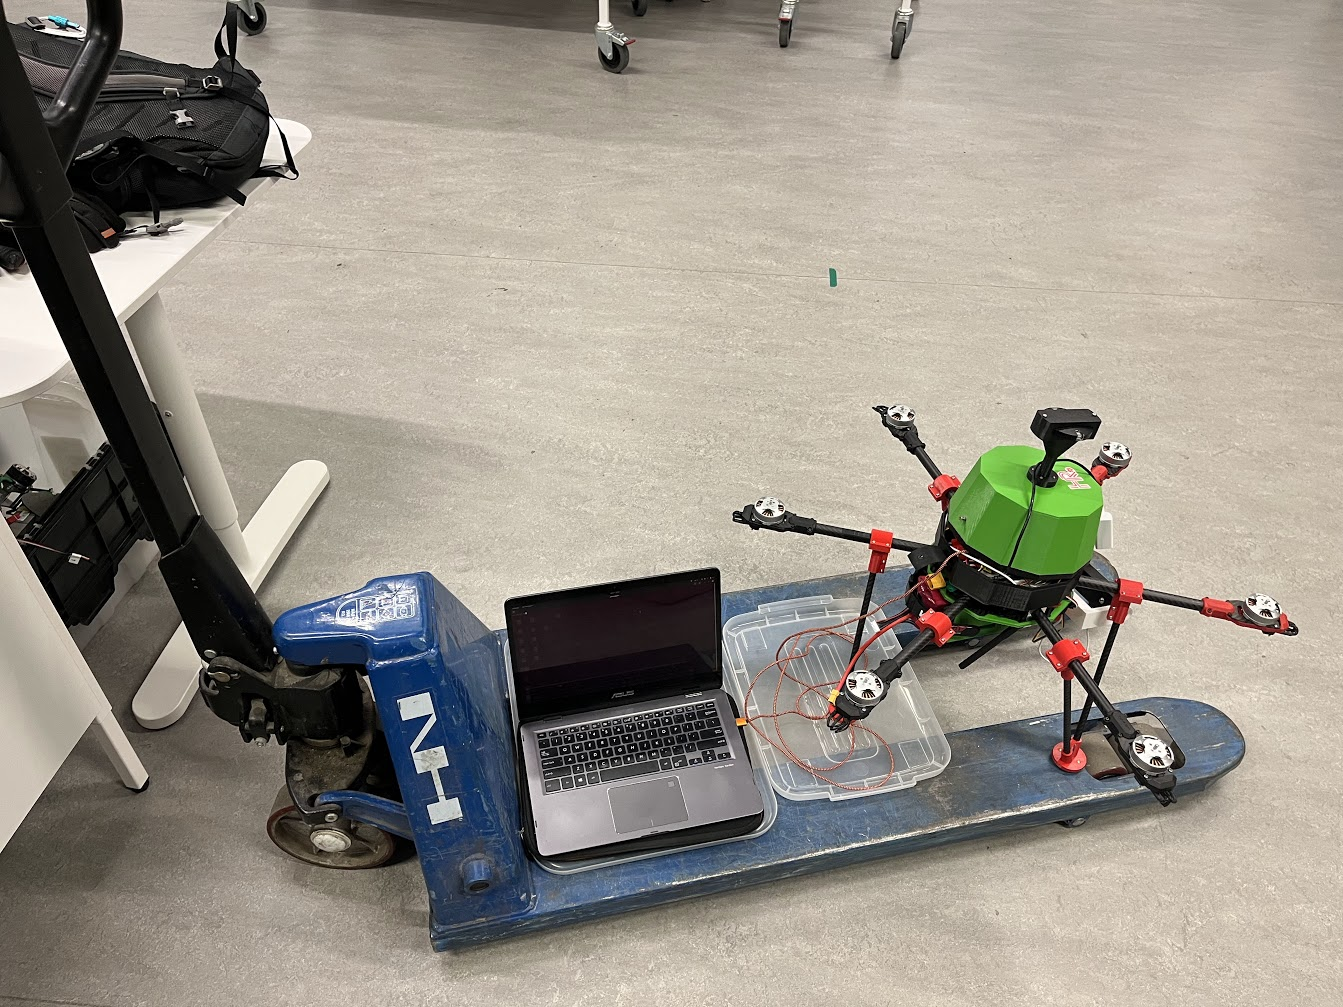
\includegraphics[width=0.75\linewidth]{./images/testing_platform.jpg}
	\caption{The testing platform, in all its glory.}
	\label{figure:testing_platform}
\end{figure}

I have marked the landmarks on the floor of V207,
beginning 1.8m from the wall going into the department of computer science.
They appear in 15x1.0m intervals, marked with pieces of electrical tape on the floor.
The distances are measured with a 3.0m, class 2 measuring tape
(although manually timestamping the landmarks in real time likely introduces more error than the small one of the
measuring tape).
At the end of the 15 meter set of points,
the track turns towards the windows 90 degrees clockwise,
and continues for 5 meters.
The 90 degree line was marked using a laser joining to the original line using a square,
as shown in Figure~\ref{figure:laser}.

\begin{figure}
	\centering
	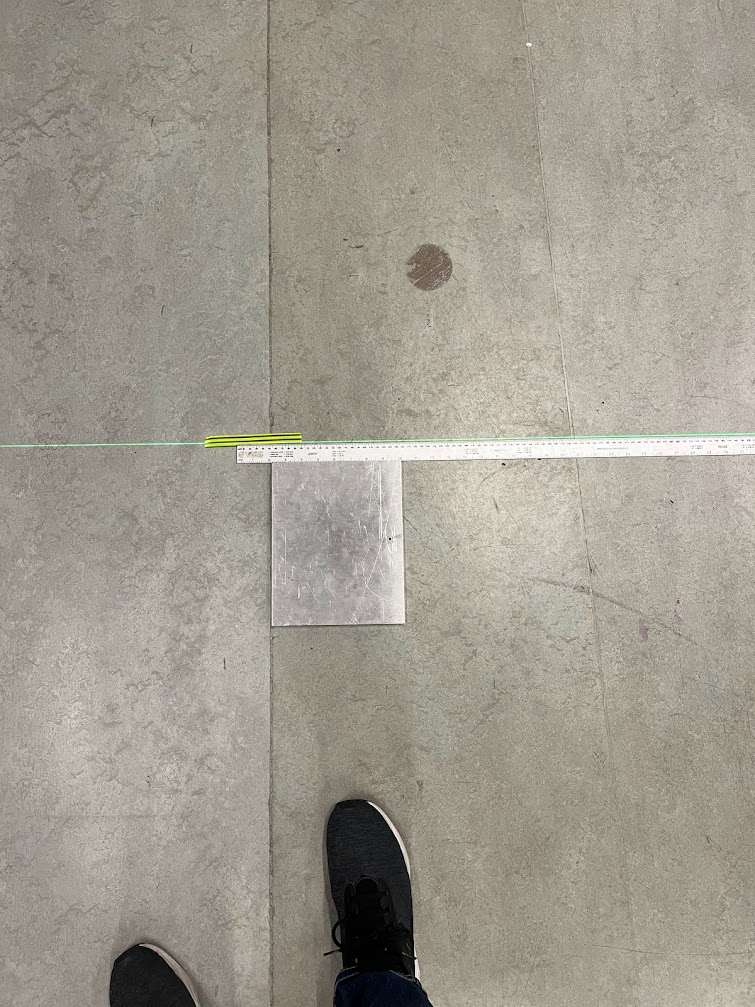
\includegraphics[width=0.75\linewidth]{./images/laser.jpg}
	\caption{Marking the adjoining line, and showing the self-similarity of the floor.}
	\label{figure:laser}
\end{figure}

Error rates for the systems are determined using ground truth markers that are manually timestamped
as the drone is pushed along its path.
The Cartesian distance between the ground truth and the estimated position is the error at each ground
truth point, considering only components $x,y$.
